% \documentclass[12pt, twoside]{article}
\usepackage[letterpaper, margin=1in, headsep=0.2in]{geometry}
\setlength{\headheight}{0.6in}
%\usepackage[english]{babel}
\usepackage[utf8]{inputenc}
\usepackage{microtype}
\usepackage{amsmath}
\usepackage{amssymb}
%\usepackage{amsfonts}
\usepackage[nomessages]{fp} %\FPeval{\var-name}{2*sin(pi/6)}
\usepackage{siunitx} %units in math. eg 20\milli\meter
\usepackage{yhmath} % for arcs, overparenth command
\usepackage{tikz} %graphics
\usetikzlibrary{quotes, angles, arrows, arrows.meta}
\usepackage{graphicx} %consider setting \graphicspath{{images/}}
\usepackage{parskip} %no paragraph indent
\usepackage{enumitem}
\usepackage{multicol}
\usepackage{venndiagram}

\usepackage{fancyhdr}
\pagestyle{fancy}
\fancyhf{}
\renewcommand{\headrulewidth}{0pt} % disable the underline of the header
\raggedbottom
\hfuzz=2mm %suppresses overfull box warnings

\usepackage{hyperref}

\fancyhead[LE]{\thepage}
\fancyhead[RO]{\thepage \\ Name: \hspace{4cm} \,\\}
\fancyhead[LO]{BECA / Dr. Huson / Geometry\\*  Learning Trajectories \\* 2022-2023}

\begin{document}

\subsubsection*{Proof Trajectory}
\begin{enumerate}
\item Given $\triangle ABC$ and $\triangle DEC$ with $\angle B \cong \angle E$. $C$ is the midpoint of $\overline{BE}$.\\ Prove $\triangle ABC \cong \triangle DEC$.\\[0.5cm]
 \begin{tikzpicture}
     \draw [thick]
       (-1,2)node[right]{$B$}--
       (1,-2)node[left]{$E$}--
       (4,0)node[right]{$D$}--
       (0,0)node[below left]{$C$}--
       (-4,0)node[left]{$A$}--cycle;
   \end{tikzpicture}
 \begin{multicols}{2}
   \underline{Statement} \\
   \underline{Reason}
 \end{multicols}
 \begin{multicols}{2}
   \raggedcolumns
   \begin{enumerate}[label={\arabic*)}]
     \item \rule{4cm}{0.15mm} \vspace{0.3cm}
     \item \rule{4cm}{0.15mm} \vspace{0.3cm}
     \item \rule{4cm}{0.15mm} \vspace{0.3cm}
     \item $\angle BCA \cong \angle ECD$  \vspace{0.3cm}
     \item \rule{4cm}{0.15mm} \vspace{0.3cm}
     \item $\triangle ABC \cong \triangle DEC$ \vspace{0.3cm}
   \end{enumerate}
   \begin{enumerate}[label={\arabic*)}]
     \item Given \vspace{0.3cm}
     \item Given \vspace{0.3cm}
     \item Given \vspace{0.3cm}
     \item \rule{4cm}{0.15mm} \vspace{0.3cm}
     \item Definition of a midpoint \vspace{0.3cm}
     \item \rule{4cm}{0.15mm} \vspace{0.3cm}
   \end{enumerate}
 \end{multicols} %\vspace{0.5cm}

 \subsubsection*{List of theorem/situations for $\triangle \cong$ proofs}
 \begin{itemize}
  \item Vertical angles w segment bisectors
  \item Transversal corresponding
  \item Transversal with shared side on transversal
  \item Two inscribed in circle with vertical angles
  \item Inscribed in circle triangle with external angle, showing arc measure relationship
  \item Rotate triangle
 \end{itemize}
  
  
\newpage
\item Given $\triangle ABP$ and $\triangle JKP$ with $\angle B \cong \angle K$. $P$ bisects $\overline{AJ}$. Prove $\triangle ABP \cong \triangle JKP$.\\[0.5cm]
  \begin{tikzpicture}
    \draw [thick]
      (0.5,-2)node[right]{$B$}--
      (-0.5,2)node[left]{$K$}--
      (4,0)node[right]{$J$}--
      (0,0)node[below left]{$P$}--
      (-4,0)node[left]{$A$}--cycle;
  \end{tikzpicture}
  \begin{multicols}{2}
    \underline{Statement} \\
    \underline{Reason}
  \end{multicols}
  \begin{multicols}{2}
  \raggedcolumns
  \begin{enumerate}[label={\arabic*)}]
    \item $\triangle ABP$, $\triangle JKP$ \vspace{0.3cm}
    \item \rule{4cm}{0.15mm} \vspace{0.3cm}
    \item \rule{4cm}{0.15mm} \vspace{0.3cm}
    \item $\angle APB \cong \angle JPK$  \vspace{0.3cm}
    \item \rule{4cm}{0.15mm} \vspace{0.3cm}
    \item $\triangle ABP \cong \triangle JKP$ \vspace{0.3cm}
  \end{enumerate}
  \begin{enumerate}[label={\arabic*)}]
    \item Given \vspace{0.3cm}
    \item Given \vspace{0.3cm}
    \item Given \vspace{0.3cm}
    \item \rule{4cm}{0.15mm} \vspace{0.3cm}
    \item Definition of a bisector \vspace{0.3cm}
    \item \rule{4cm}{0.15mm} \vspace{0.3cm}
  \end{enumerate}
  \end{multicols}

\newpage
\item Given $\triangle QRP$ and $\triangle STP$ with $\overline{QP} \cong \overline{SP}$. $P$ is the midpoint $\overline{RT}$.\\ Prove $\triangle QRP \cong \triangle STP$.\\[0.5cm]
 \begin{tikzpicture}
     \draw [thick]
       (-1,2)node[right]{$R$}--
       (1,-2)node[left]{$T$}--
       (4,0)node[right]{$S$}--
       (0,0)node[below left]{$P$}--
       (-4,0)node[left]{$Q$}--cycle;
   \end{tikzpicture}
  \begin{multicols}{2}
    \underline{Statement} \\
    \underline{Reason}
  \end{multicols}
  \begin{multicols}{2}
   \raggedcolumns
   \begin{enumerate}[label={\arabic*)}]
     \item $\triangle QRP$, $\triangle STP$ \vspace{0.3cm}
     \item \rule{4cm}{0.15mm} \vspace{0.3cm}
     \item \rule{4cm}{0.15mm} \vspace{0.3cm}
     \item $\angle QPR \cong \angle SPT$  \vspace{0.3cm}
     \item \rule{4cm}{0.15mm} \vspace{0.3cm}
     \item $\triangle QRP \cong \triangle STP$ \vspace{0.3cm}
   \end{enumerate}
   \begin{enumerate}[label={\arabic*)}]
     \item Given \vspace{0.3cm}
     \item Given \vspace{0.3cm}
     \item Given \vspace{0.3cm}
     \item \rule{4cm}{0.15mm} \vspace{0.3cm}
     \item Definition of a midpoint \vspace{0.3cm}
     \item \rule{4cm}{0.15mm} \vspace{0.3cm}
   \end{enumerate}
 \end{multicols} \vspace{0.5cm}

\newpage
\item The transversal $\overleftrightarrow{MPR}$ intersects two parallel lines,  $\overleftrightarrow{PQ} || \overleftrightarrow{MN}$. Given $\angle PRQ \cong \angle MPN$ and $P$ bisects $\overline{MR}$. \\Prove $\triangle MPN \cong \triangle PRQ$.
  \begin{center}
  \begin{tikzpicture}[scale=1.4]
    \draw [<->, thick] (-1,0)--(0,0)--(3,0);
    \draw [<->, thick] (-0.5,-0.5)--(4,4)--(4.5,4.5);
    \draw [<->, thick] (1,2)--(4.5,2);
    \draw [-, thick] (4,4)--(3.5, 2);
    \draw [-, thick] (2,2)--(1.5,0);
    \draw [fill] (4,4) circle [radius=0.05] node[above left]{$R$};
    \draw [fill] (3.5, 2) circle [radius=0.05] node[below]{$Q$};
    \draw [fill] (2,2) circle [radius=0.05] node[above left]{$P$};
    \draw [fill] (0,0) circle [radius=0.05] node[above left]{$M$};
    \draw [fill] (1.5,0) circle [radius=0.05] node[below]{$N$};
  \end{tikzpicture}
  \end{center}
  \begin{multicols}{2}
    \underline{Statement} \\
    \underline{Reason}
  \end{multicols}
  \begin{multicols}{2}
    \raggedcolumns
    \begin{enumerate}[label={\arabic*)}]
      \item \rule{4cm}{0.15mm} \vspace{0.3cm}
      \item \rule{4cm}{0.15mm} \vspace{0.3cm}
      \item \rule{4cm}{0.15mm} \vspace{0.3cm}
      \item $\angle RPQ \cong \angle PMN$ \vspace{0.3cm}
      \item \rule{4cm}{0.15mm} \vspace{0.3cm}
      \item $\triangle MPN \cong \triangle PRQ$  \vspace{0.3cm}
    \end{enumerate}
    \begin{enumerate}[label={\arabic*)}]
      \item Given \vspace{0.3cm}
      \item Given \vspace{0.3cm}
      \item Given \vspace{0.3cm}
      \item \rule{4cm}{0.15mm} \vspace{0.3cm}
      \item Definition of a bisector \vspace{0.3cm}
      \item \rule{4cm}{0.15mm} \vspace{0.3cm}
    \end{enumerate}
  \end{multicols}

\newpage  
\item Given two parallel lines are intersected by a transversal,  $\overleftrightarrow{MD} || \overleftrightarrow{BC}$. $m\angle AMD =4x+5$ and $m\angle MBC=5x-7$. Find $m\angle AMD$.\\[1cm]
   \begin{tikzpicture}[scale=1.1]
     \draw [<->, thick] (-1,0)--(0,0)--(4,0);
     \draw [<->, thick] (-0.5,-0.5)--(4,4)--(4.5,4.5);
     \draw [<->, thick] (1,2)--(5, 2)--(5.5,2);
     \draw [fill] (4,4) circle [radius=0.05] node[above left]{$A$};
     \draw [fill] (5, 2) circle [radius=0.05] node[below]{$D$};
     \draw [fill] (2,2) circle [radius=0.05] node[above left]{$M$};
     \draw [fill] (0,0) circle [radius=0.05] node[above left]{$B$};
     \draw [fill] (3,0) circle [radius=0.05] node[below]{$C$};
   \end{tikzpicture} \vspace{1cm}

  \item In the diagram above, the point $M$ bisects $\overline{AB}$. If $AM=4$ find $AB$. \vspace{2cm}

 \item Given $\triangle ABC$ and $\triangle EFG$ with $\overline{AB} \cong \overline{EF}$, $\overline{BC} \cong \overline{FG}$, and $\overline{AC} \cong \overline{EG}$. \\Prove $\triangle ABC \cong \triangle EFG$ (by filling in the blanks below)\\[0.5cm]
   \begin{tikzpicture}
       \draw [thick]
         (2,0)node[below]{$A$}--
         (8,0)node[below]{$B$}--
         (4,3)node[above]{$C$} --(2,0);
     \end{tikzpicture}
     \begin{tikzpicture}%[scale=0.7]
       \draw [thick]%(0,0)node[below]{$A$}--
       (2,0)node[below]{$E$}--
       (8,0)node[below]{$F$}--
       (4,3)node[above]{$G$} --(2,0);
   \end{tikzpicture}
   \begin{multicols}{2}
     \underline{Statement} \\
     \underline{Reason}
   \end{multicols}
   \begin{multicols}{2}
     \raggedcolumns
     \begin{enumerate}[label={\arabic*)}]
       \item $\triangle ABC$, $\triangle EFG$
       \item $\overline{AB} \cong \overline{EF}$
       \item $\overline{BC} \cong \overline{FG}$, $\overline{AC} \cong \overline{EG}$
       \item $\triangle ABC \cong \triangle EFG$ \\
     \end{enumerate}
     \begin{enumerate}[label={\arabic*)}]
       \item Given
       \item \rule{4cm}{0.15mm}
       \item \rule{4cm}{0.15mm}
       \item \rule{4cm}{0.15mm}
     \end{enumerate}
   \end{multicols}

\newpage
\item Given two parallel lines intersect a transversal,  $\overleftrightarrow{MD} || \overleftrightarrow{BC}$. Given $\overline{MD} \cong \overline{BC}$ and $M$ is the midpoint of $\overline{AB}$. \\Prove $\triangle ADM \cong \triangle MCB$.
  \begin{center}
  \begin{tikzpicture}[scale=1.4]
    \draw [<->, thick] (-1,0)--(0,0)--(4,0);
    \draw [<->, thick] (-0.5,-0.5)--(4,4)--(4.5,4.5);
    \draw [<->, thick] (1,2)--(5, 2)--(5.5,2);
    \draw [-, thick] (4,4)--(5, 2);
    \draw [-, thick] (2,2)--(3,0);
    \draw [fill] (4,4) circle [radius=0.05] node[above left]{$A$};
    \draw [fill] (5, 2) circle [radius=0.05] node[below]{$D$};
    \draw [fill] (2,2) circle [radius=0.05] node[above left]{$M$};
    \draw [fill] (0,0) circle [radius=0.05] node[above left]{$B$};
    \draw [fill] (3,0) circle [radius=0.05] node[below]{$C$};
  \end{tikzpicture}
  \end{center}
  \begin{multicols}{2}
    \underline{Statement} \\
    \underline{Reason}
  \end{multicols}
  \begin{multicols}{2}
    \raggedcolumns
    \begin{enumerate}[label={\arabic*)}]
      \item $\overleftrightarrow{MD} || \overleftrightarrow{BC}$ \vspace{0.3cm}
      \item $M$ is the midpoint of $\overline{AB}$ \vspace{0.3cm}
      \item \rule{2cm}{0.15mm} $\cong \overline{BC}$ \vspace{0.3cm}
      \item $\angle AMD \cong \angle MBC$ \vspace{0.3cm}
      \item \rule{2cm}{0.15mm} $\cong \overline{AM}$ \vspace{0.3cm}
      \item $\triangle ADM \cong \triangle MCB$  \vspace{0.3cm}
    \end{enumerate}
    \begin{enumerate}[label={\arabic*)}]
      \item \rule{4cm}{0.15mm} \vspace{0.3cm}
      \item \rule{4cm}{0.15mm} \vspace{0.3cm}
      \item Given \vspace{0.3cm}
      \item \rule{4cm}{0.15mm} \vspace{0.3cm}
      \item Definition of a midpoint \vspace{0.3cm}
      \item \rule{4cm}{0.15mm} \vspace{0.3cm}
    \end{enumerate}
  \end{multicols}

\newpage
\item Given $\triangle ABC$ and $\triangle EFG$ with $\angle A \cong \angle E$, $\overline{AB} \cong \overline{EF}$, and $\overline{AC} \cong \overline{EG}$. Prove $\triangle ABC \cong \triangle EFG$.\\[0.5cm]
  \begin{tikzpicture}
      \draw [thick]
        (2,0)node[below]{$A$}--
        (8,0)node[below]{$B$}--
        (4,3)node[above]{$C$} --(2,0);
    \end{tikzpicture}
    \begin{tikzpicture}%[scale=0.7]
      \draw [thick]%(0,0)node[below]{$A$}--
      (2,0)node[below]{$E$}--
      (8,0)node[below]{$F$}--
      (4,3)node[above]{$G$} --(2,0);
  \end{tikzpicture}
  \begin{multicols}{2}
    \underline{Statement} \\
    \underline{Reason}
  \end{multicols}
  \begin{multicols}{2}
    \raggedcolumns
    \begin{enumerate}[label={\arabic*)}]
      \item $\triangle ABC$, $\triangle EFG$
      \item $\angle A \cong \angle E$
      \item $\overline{AB} \cong \overline{EF}$, and $\overline{AC} \cong \overline{EG}$
      \item $\triangle ABC \cong \triangle EFG$ \\
    \end{enumerate}
    \begin{enumerate}[label={\arabic*)}]
      \item Given
      \item \rule{4cm}{0.15mm}
      \item \rule{4cm}{0.15mm}
      \item \rule{4cm}{0.15mm}
    \end{enumerate}
  \end{multicols}

\newpage
\item Given $\triangle ABP$ and $\triangle JKP$ with $\angle A \cong \angle J$ and $\overline{AP} \cong \overline{JP}$. Prove $\triangle ABP \cong \triangle JKP$.\\[0.5cm]
  \begin{tikzpicture}
      \draw [thick]
        (-2,-1)node[left]{$A$}--
        (3,3)node[right]{$K$}--
        (2,-1)node[right]{$J$}--
        (0,0.6)node[below]{$P$}--
        (-3,3)node[left]{$B$}--(-2,-1);
    \end{tikzpicture}
  \begin{multicols}{2}
    \underline{Statement} \\
    \underline{Reason}
  \end{multicols}
  \begin{multicols}{2}
    \raggedcolumns
    \begin{enumerate}[label={\arabic*)}]
      \item $\triangle ABC$, $\triangle JKP$
      \item \rule{4cm}{0.15mm}%$\angle A \cong \angle J$ and $\overline{AP} \cong \overline{JP}$ %\vspace{0.4cm}
      \item $\angle APB \cong \angle JPK$ 
      \item $\triangle ABP \cong \triangle JKP$
    \end{enumerate}
    \begin{enumerate}[label={\arabic*)}]
      \item Given
      \item Given
      \item \rule{4cm}{0.15mm}
      \item \rule{4cm}{0.15mm}
    \end{enumerate}
  \end{multicols}


\end{enumerate}
\end{document}
